\section{Results}\label{sec:results}

\subsection{Two portfolios of very different size and profile}\label{sec:res-profile}
Assessed debt is \pctCdaAssessed\% of the \vat{} CDAs and \pctStockAssessed\% of the stock (Table~\ref{tab:profile}).
The mean legal-entity assessed CDA is BRL~\meanValueAssessed, against BRL~\meanValueDeclared{} for declared debt; the medians are BRL~\medianValueAssessed{} and BRL~\medianValueDeclared.
By the thresholds fixed in Section~\ref{sec:method}, the difference in value between the two origins is substantial ($|r|=\rBisValue$), and so is the difference in age ($|r|=\rBisAge$; median \medianAgeAssessed{} against \medianAgeDeclared{} years).
\pctAnyPaymentAssessed\% of assessed and \pctAnyPaymentDeclared\% of declared CDAs in the panel received any payment; the median time to the first payment is \yearsFirstPaymentAssessed{} and \yearsFirstPaymentDeclared{} years.
The difference in the CDA recovery rate is non-negligible but below the substantial threshold ($|r|=\rBisRate$; Kruskal--Wallis $H={}$\kwRateH{} across the five raw types).

\begin{table}[H]\centering\small
\caption{Profile of the two origins. Value, age and filing: December 2025 snapshot, legal entities; payment: 2016--2025 panel.}\label{tab:profile}
% generated by projects/macro/notebooks/articles/icms_declarado_autuado.ipynb; do not edit by hand
% Profile of the two origins; value, age and filing in the December 2025 snapshot (legal entities); payment in the 2016-2025 panel
\begin{tabular}{lrr}
\toprule
measure & Assessed & Declared \\
\midrule
CDAs, all debtors (Dec 2025) & 59,536 & 2,254,464 \\
Stock, BRL bn (Dec 2025) & 313.3 & 116.4 \\
Share of VAT (ICMS) stock, \% & 72.9 & 27.1 \\
Mean CDA value, BRL & 5,322,754 & 51,643 \\
Median CDA value, BRL & 596,311 & 7,334 \\
Median age, years & 9.26 & 4.61 \\
CDAs filed in court, \% & 88.4 & 69.7 \\
Stock filed in court, \% & 91.5 & 94.2 \\
CDAs with any payment, \% (2016-2025) & 14.4 & 25.9 \\
Median years to first payment & 3.34 & 0.19 \\
\bottomrule
\end{tabular}

\end{table}

\subsection{Concentration}\label{sec:res-conc}
Across all \vat{} debt, the largest 1\% of CDAs hold \topOneCdaVat\% of the stock, and \kFiftyDebtorVat{} debtors owe half of it.
Half of the assessed stock is owed by \kFiftyDebtorAssessed{} debtors and half of the declared stock by \kFiftyDebtorDeclared{} (Table~\ref{tab:conc}, Figure~\ref{fig:conc}).
Within each origin, the largest 1\% of debtors hold \topOneDebtorDeclared\% of the declared stock and \topOneDebtorAssessed\% of the assessed stock (Gini \giniDebtorDeclared{} and \giniDebtorAssessed).
The two measures point in different directions because the declared portfolio has many more debtors, so the same fraction means many more firms.
\discutir{joint reading of the two concentration measures}

\begin{table}[H]\centering\small
\caption{Concentration of the stock by debtor (CNPJ root), December 2025.}\label{tab:conc}
\resizebox{\linewidth}{!}{% generated by projects/macro/notebooks/articles/icms_declarado_autuado.ipynb; do not edit by hand
% Concentration of the stock by debtor (CNPJ root), December 2025, all debtors with a CNPJ
\begin{tabular}{lrrrrrrr}
\toprule
group & debtors & stock (BRL bn) & Gini & top 0.1\% (\%) & top 1\% (\%) & top 10\% (\%) & k50 \\
\midrule
VAT (ICMS), all types & 195,925 & 427.9 & 0.961 & 35.3 & 68.6 & 95.1 & 550 \\
Assessed (ICMS Autuação) & 29,328 & 311.3 & 0.896 & 18.3 & 49.5 & 85.2 & 302 \\
Declared (ICMS Declarado) & 177,600 & 116.4 & 0.944 & 29.5 & 58.9 & 92.3 & 982 \\
Assessed origin (Autuação + Simples Nacional) & 29,855 & 311.4 & 0.898 & 18.6 & 49.8 & 85.4 & 303 \\
\bottomrule
\end{tabular}
}
\end{table}

\begin{figure}[H]\centering
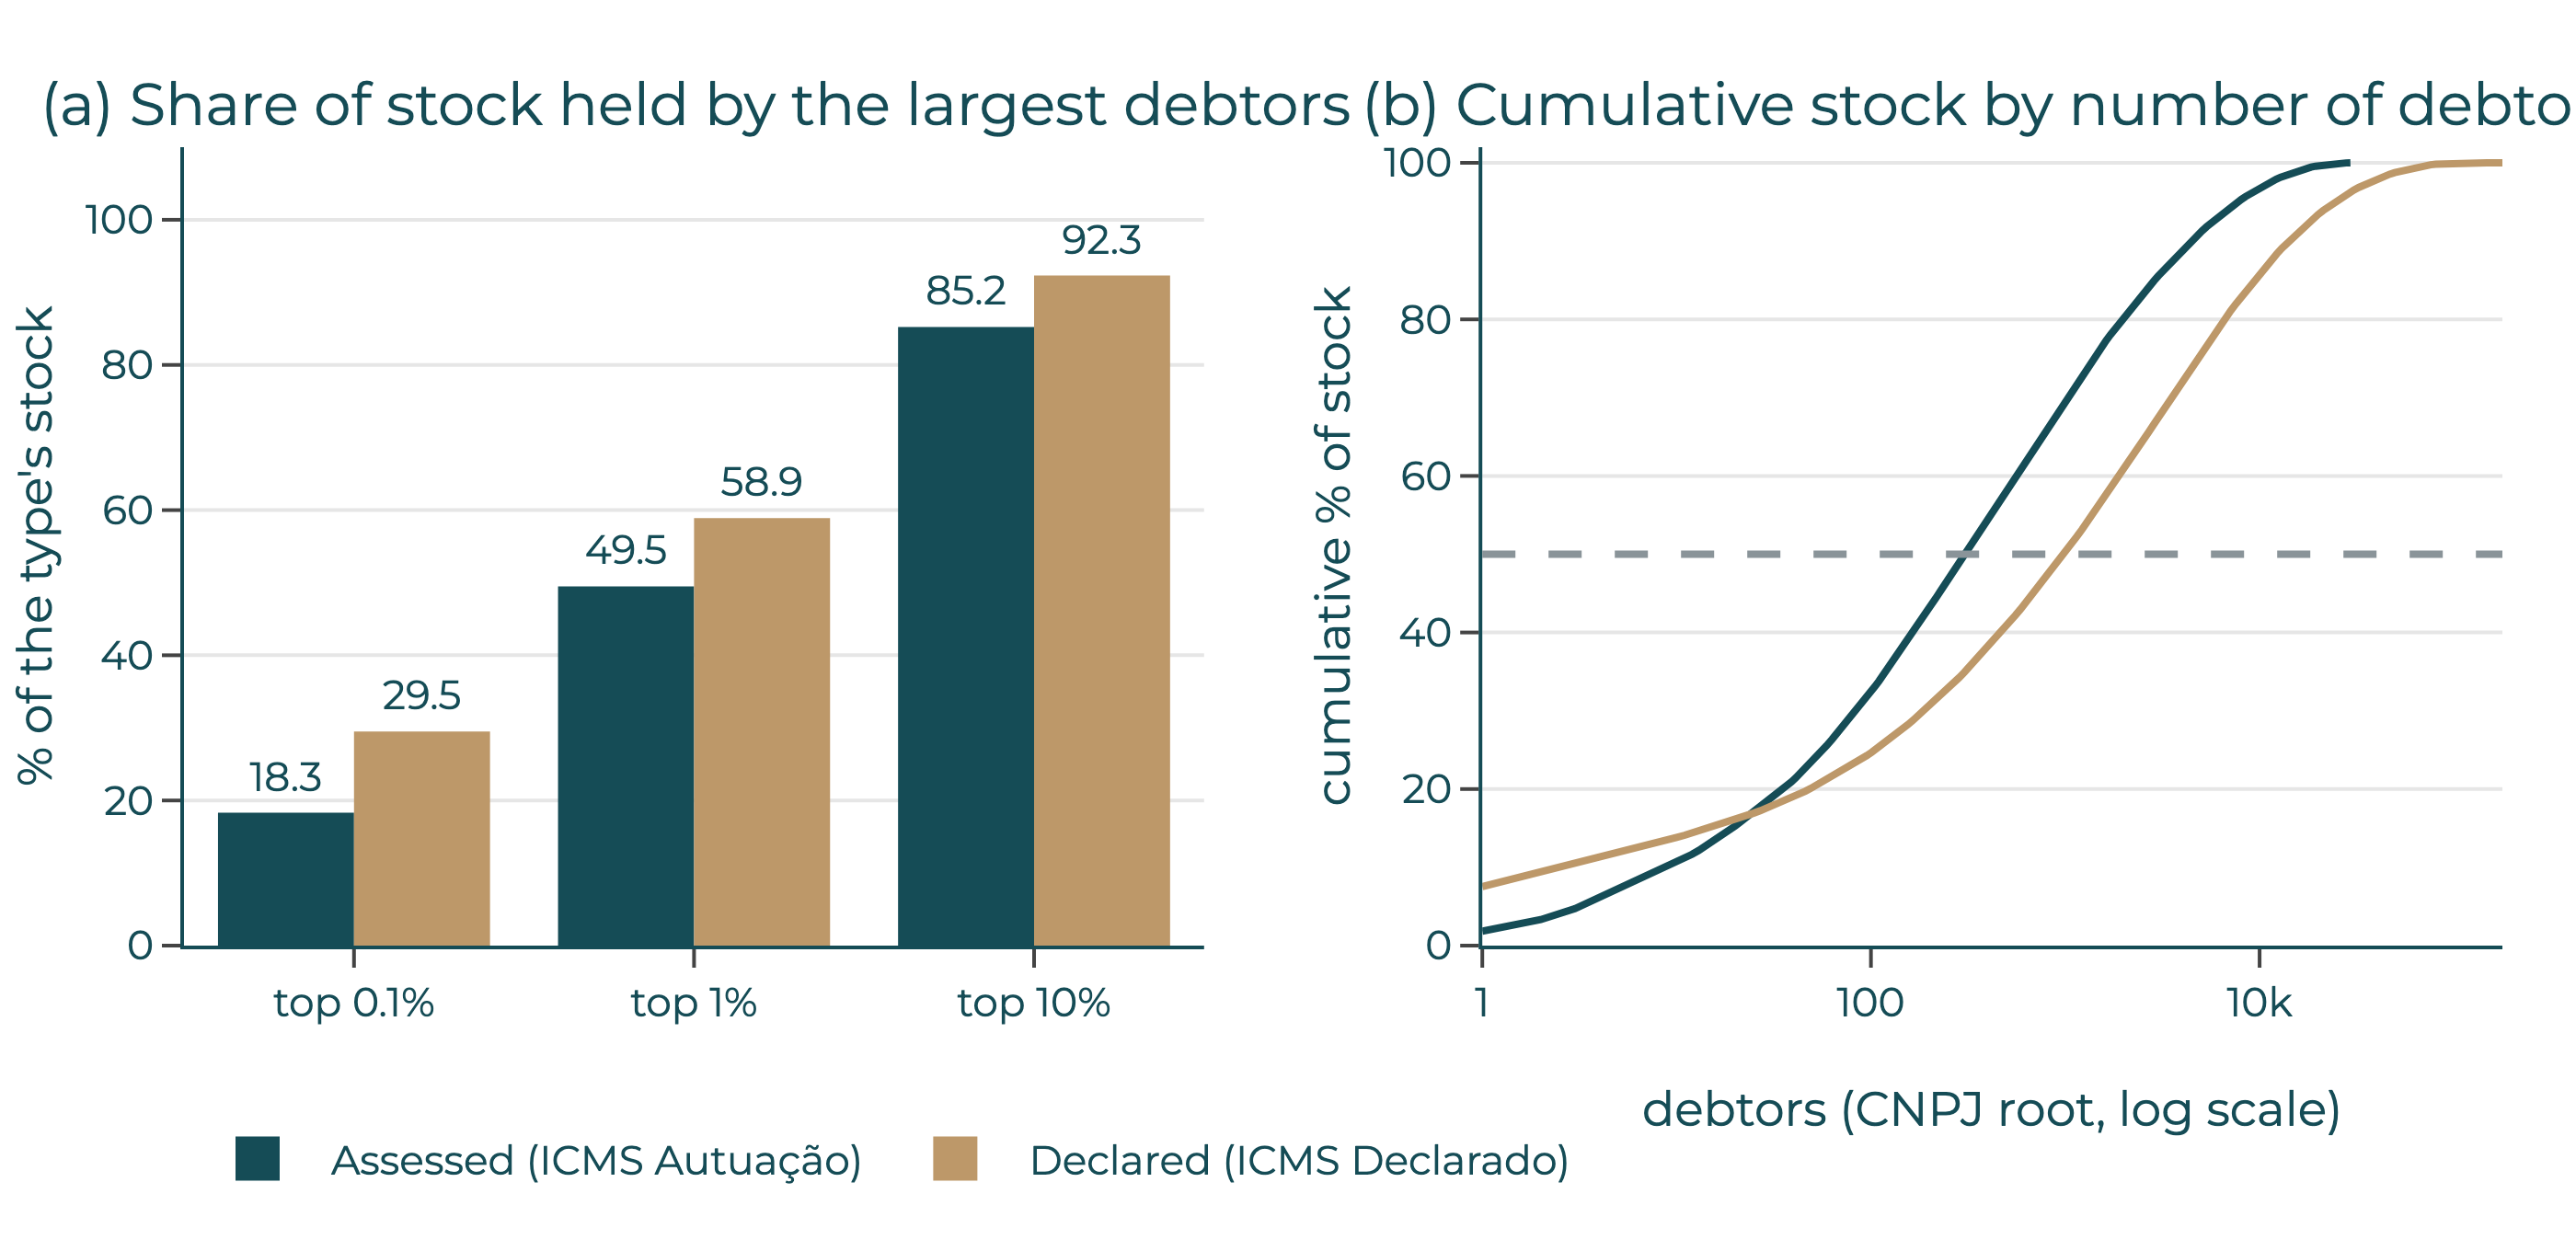
\includegraphics[width=\linewidth]{figures/fig_concentration_origin.png}
\caption{Share of each origin's stock held by the largest debtors (a) and cumulative stock by number of debtors, log scale (b). December 2025.}\label{fig:conc}
\end{figure}

\subsection{Recovery over time, and three open questions}\label{sec:res-series}
From 2016 to 2025, the annual recovery rate ranged from \rateMinDeclared\% (\rateMinYearDeclared) to \rateMaxDeclared\% (\rateMaxYearDeclared) for declared debt and from \rateMinAssessed\% (\rateMinYearAssessed) to \rateMaxAssessed\% (\rateMaxYearAssessed) for assessed debt (Figure~\ref{fig:series}).
In 2025 the rates were \rateTwentyFiveDeclared\% and \rateTwentyFiveAssessed\%.

The assessed series has three features this paper does not explain, registered as open research questions:
\begin{itemize}
\item \textbf{RQ-A, the 2020 fall.} The number of assessed CDAs in the panel falls from \cdaAssessedNineteen{} in 2019 to \cdaAssessedTwenty{} in 2020. Is it an artefact of the missing October--December 2020 snapshots, or a change in the assessed portfolio?
\item \textbf{RQ-B, the 2019 and 2024 peaks.} Assessed payments reach BRL~\paidAssessedNineteen{} billion in 2019 and BRL~\paidAssessedTwentyFour{} billion in 2024. Are the peaks related to instalment programmes or settlement agreements in those years, or to a few very large payments? Answering requires payment-level timing and the programme rules.
\item \textbf{RQ-C, data.} Do the comparisons by origin hold when the panel is re-run on a \texttt{DEBITO} table without missing and partial snapshots?
\end{itemize}
No cause is asserted for any of them; the series will be re-run once the missing snapshots are restored.

\begin{figure}[H]\centering
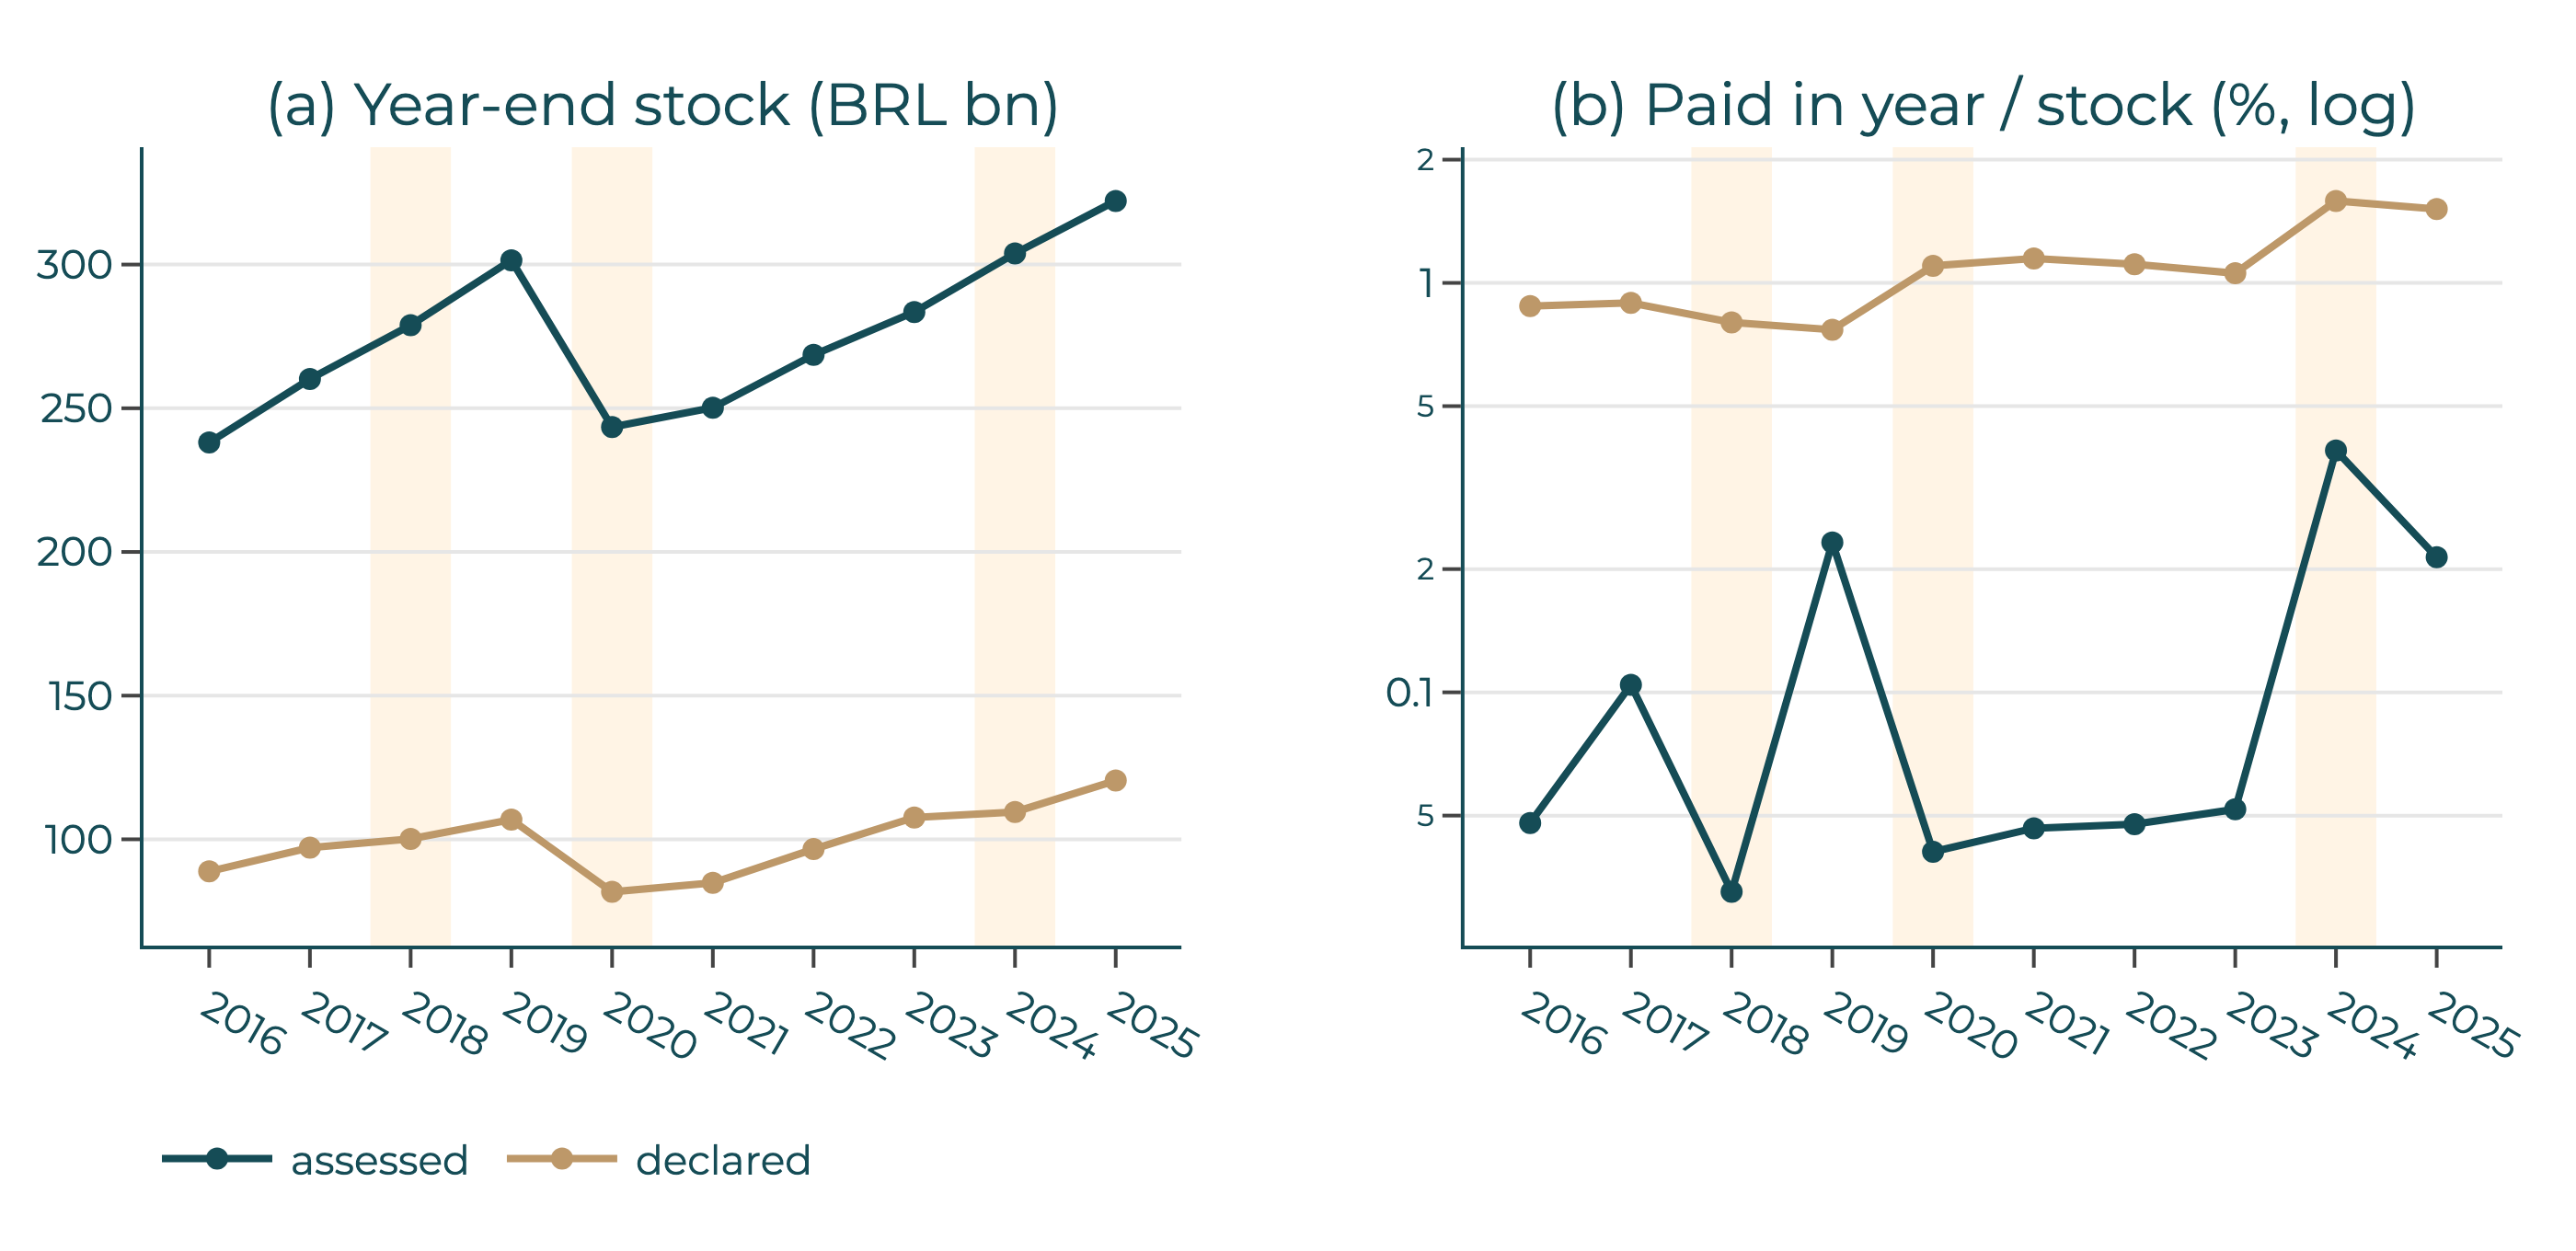
\includegraphics[width=\linewidth]{figures/fig_annual_series_origin.png}
\caption{Year-end stock (a) and annual recovery rate, log scale (b), by origin, legal entities, 2016--2025. Shaded years have missing (2018, 2020) or partial (2024) snapshots.}\label{fig:series}
\end{figure}

\subsection{The largest debts}\label{sec:res-top}
Among the largest 1\% of legal-entity CDAs (\kmN{} CDAs, at least BRL~\kmMinValueMn{} million each, BRL~\kmSumBn{} billion in total), \topOnePctCdaAssessed\% are assessed and they carry \topOnePctValueAssessed\% of the value.
In the rest of the portfolio (outside the top 1\%), \restOnePctCdaAssessed\% of the CDAs are assessed, with \restOnePctValueAssessed\% of the value (Table~\ref{tab:top}).
In the finer cut of the top 0.1\%, \topTenthPctCdaAssessed\% of the CDAs are assessed.

\begin{table}[H]\centering\small
\caption{Assessed share among the largest legal-entity CDAs, December 2025. The rest is everything outside the top 1\%.}\label{tab:top}
% generated by projects/macro/notebooks/articles/icms_declarado_autuado.ipynb; do not edit by hand
% Assessed share among the largest legal-entity CDAs, December 2025; rest = outside the top 1%
\begin{tabular}{lrrr}
\toprule
set of CDAs & assessed CDAs & assessed share of CDAs (\%) & assessed share of value (\%) \\
\midrule
top 0.1\% & 2,180 & 93.9 & 93.5 \\
top 1\% & 18,283 & 78.7 & 90.7 \\
rest (outside top 1\%) & 41,011 & 1.8 & 16.6 \\
\bottomrule
\end{tabular}

\end{table}

Inside the top 1\%, the silhouette at $k=4$ is \kmSilEuclid{} (Euclidean) and \kmSilGower{} (Gower).
The four groups split mainly by origin (Table~\ref{tab:km}); the largest, G1, has \kmGOnePctCda\% of the CDAs and \kmGOnePctValue\% of the value.
Origin is one of the clustering inputs, so this separation is partly built in.
Without origin, the adjusted Rand index between the two partitions is \kmNoOriginAri{} (1 = same partition, 0 = chance agreement) and the origin purity of the clusters falls from \kmPurityWith\% to \kmPurityWithout\%, the level of the largest origin in the top 1\% (\kmPurityBase\%).
\discutir{whether origin should be read as the axis that separates the largest debts}

\begin{table}[H]\centering\small
\caption{K-means ($k=4$) on the top 1\% of legal-entity CDAs, December 2025. Modal labels are translated from the raw database values.}\label{tab:km}
\resizebox{\linewidth}{!}{% generated by projects/macro/notebooks/articles/icms_declarado_autuado.ipynb; do not edit by hand
% K-means (k = 4) on the top 1% of legal-entity CDAs, December 2025; modal labels translated from the raw database values
\begin{tabular}{lrrrrrrrr}
\toprule
cluster & CDAs (\%) & value (\%) & modal origin & modal situation & modal filing status & median value (BRL mn) & median age (years) & any payment (\%) \\
\midrule
G1 & 70.7 & 79.7 & assessed (100.0\%) & enrolled & filed in court & 4.69 & 10.0 & 12.5 \\
G2 & 19.6 & 8.8 & declared (100.0\%) & enrolled & filed in court & 2.47 & 9.6 & 12.0 \\
G3 & 6.4 & 6.1 & assessed (77.2\%) & enrolled & cleared for filing & 3.83 & 0.8 & 16.5 \\
G4 & 3.3 & 5.4 & assessed (94.0\%) & suspended & filed in court & 5.27 & 6.1 & 6.1 \\
\bottomrule
\end{tabular}
}
\end{table}

\subsection{Debtor firm characteristics (descriptors only)}\label{sec:res-firms}
Registration status and economic activity are measured in March 2026, after the outcomes, and describe the debtors of each origin; they are not causes.

\paragraph{Registration status.}
Firms active in March 2026 hold \stPctStockAssessedActive\% of the assessed and \stPctStockDeclaredActive\% of the declared stock; firms declared unfit (\emph{inapta}) hold \stPctStockAssessedUnfit\% and \stPctStockDeclaredUnfit\% (Table~\ref{tab:status}).
The pooled 2016--2025 recovery rate of assessed debt is \stRecoveryAssessedActive\% for active firms and \stRecoveryAssessedUnfit\% for unfit firms; for declared debt it is \stRecoveryDeclaredActive\% and \stRecoveryDeclaredUnfit\%.
In the 2016--2025 enrolment cohort, \kmPaidFiveYrAssessedActive\% of assessed CDAs of active firms had a first payment within 60 months, against \kmPaidFiveYrAssessedUnfit\% for unfit firms (Figure~\ref{fig:km}).
A firm may be closed or unfit \emph{because} of its debts, so these differences are associations.

\begin{table}[H]\centering\small
\caption{Registration status of the debtor CNPJ (RFB, March 2026) by origin. Descriptors only. KM: Kaplan--Meier share of CDAs of the 2016--2025 enrolment cohort with a first payment by 12 and 60 months; empty cells have no CDA in the cohort.}\label{tab:status}
\resizebox{\linewidth}{!}{% generated by projects/macro/notebooks/articles/icms_declarado_autuado.ipynb; do not edit by hand
% Registration status of the debtor CNPJ (RFB, March 2026) by origin, descriptors only; KM = Kaplan-Meier share with a first payment, enrolment cohort 2016-2025
\begin{tabular}{lrrrrrrr}
\toprule
origin & status (Mar 2026) & CNPJs & share of origin stock (\%) & any payment (\%) & pooled recovery (\%) & KM 12 m (\%) & KM 60 m (\%) \\
\midrule
assessed & active & 15,640 & 52.9 & 30.8 & 0.22 & 18.9 & 35.1 \\
assessed & unfit (inapta) & 9,243 & 21.7 & 5.5 & 0.01 & 2.9 & 6.8 \\
assessed & suspended & 275 & 1.2 & 14.0 & 0.02 & 8.1 & 22.3 \\
assessed & closed (baixada) & 7,625 & 24.1 & 8.0 & 0.10 & 11.4 & 22.6 \\
assessed & null (nula) & 25 & 0.0 & 5.6 & 0.00 & 2.1 & 2.1 \\
assessed & root only (status unknown) & 193 & 0.0 & 0.7 & 0.00 &  &  \\
assessed & not found in register & 138 & 0.0 & 0.7 & 0.01 &  &  \\
declared & active & 142,869 & 74.4 & 30.4 & 1.70 & 30.2 & 36.5 \\
declared & unfit (inapta) & 20,994 & 15.2 & 7.0 & 0.07 & 8.6 & 10.3 \\
declared & suspended & 806 & 0.5 & 13.9 & 0.52 & 13.1 & 16.5 \\
declared & closed (baixada) & 29,882 & 9.7 & 16.9 & 0.47 & 22.7 & 27.5 \\
declared & null (nula) & 80 & 0.1 & 10.3 & 0.11 & 10.3 & 12.5 \\
declared & root only (status unknown) & 140 & 0.1 & 1.2 & 0.01 &  &  \\
declared & not found in register & 72 & 0.0 & 0.3 & 0.00 &  &  \\
\bottomrule
\end{tabular}
}
\end{table}

\begin{figure}[H]\centering
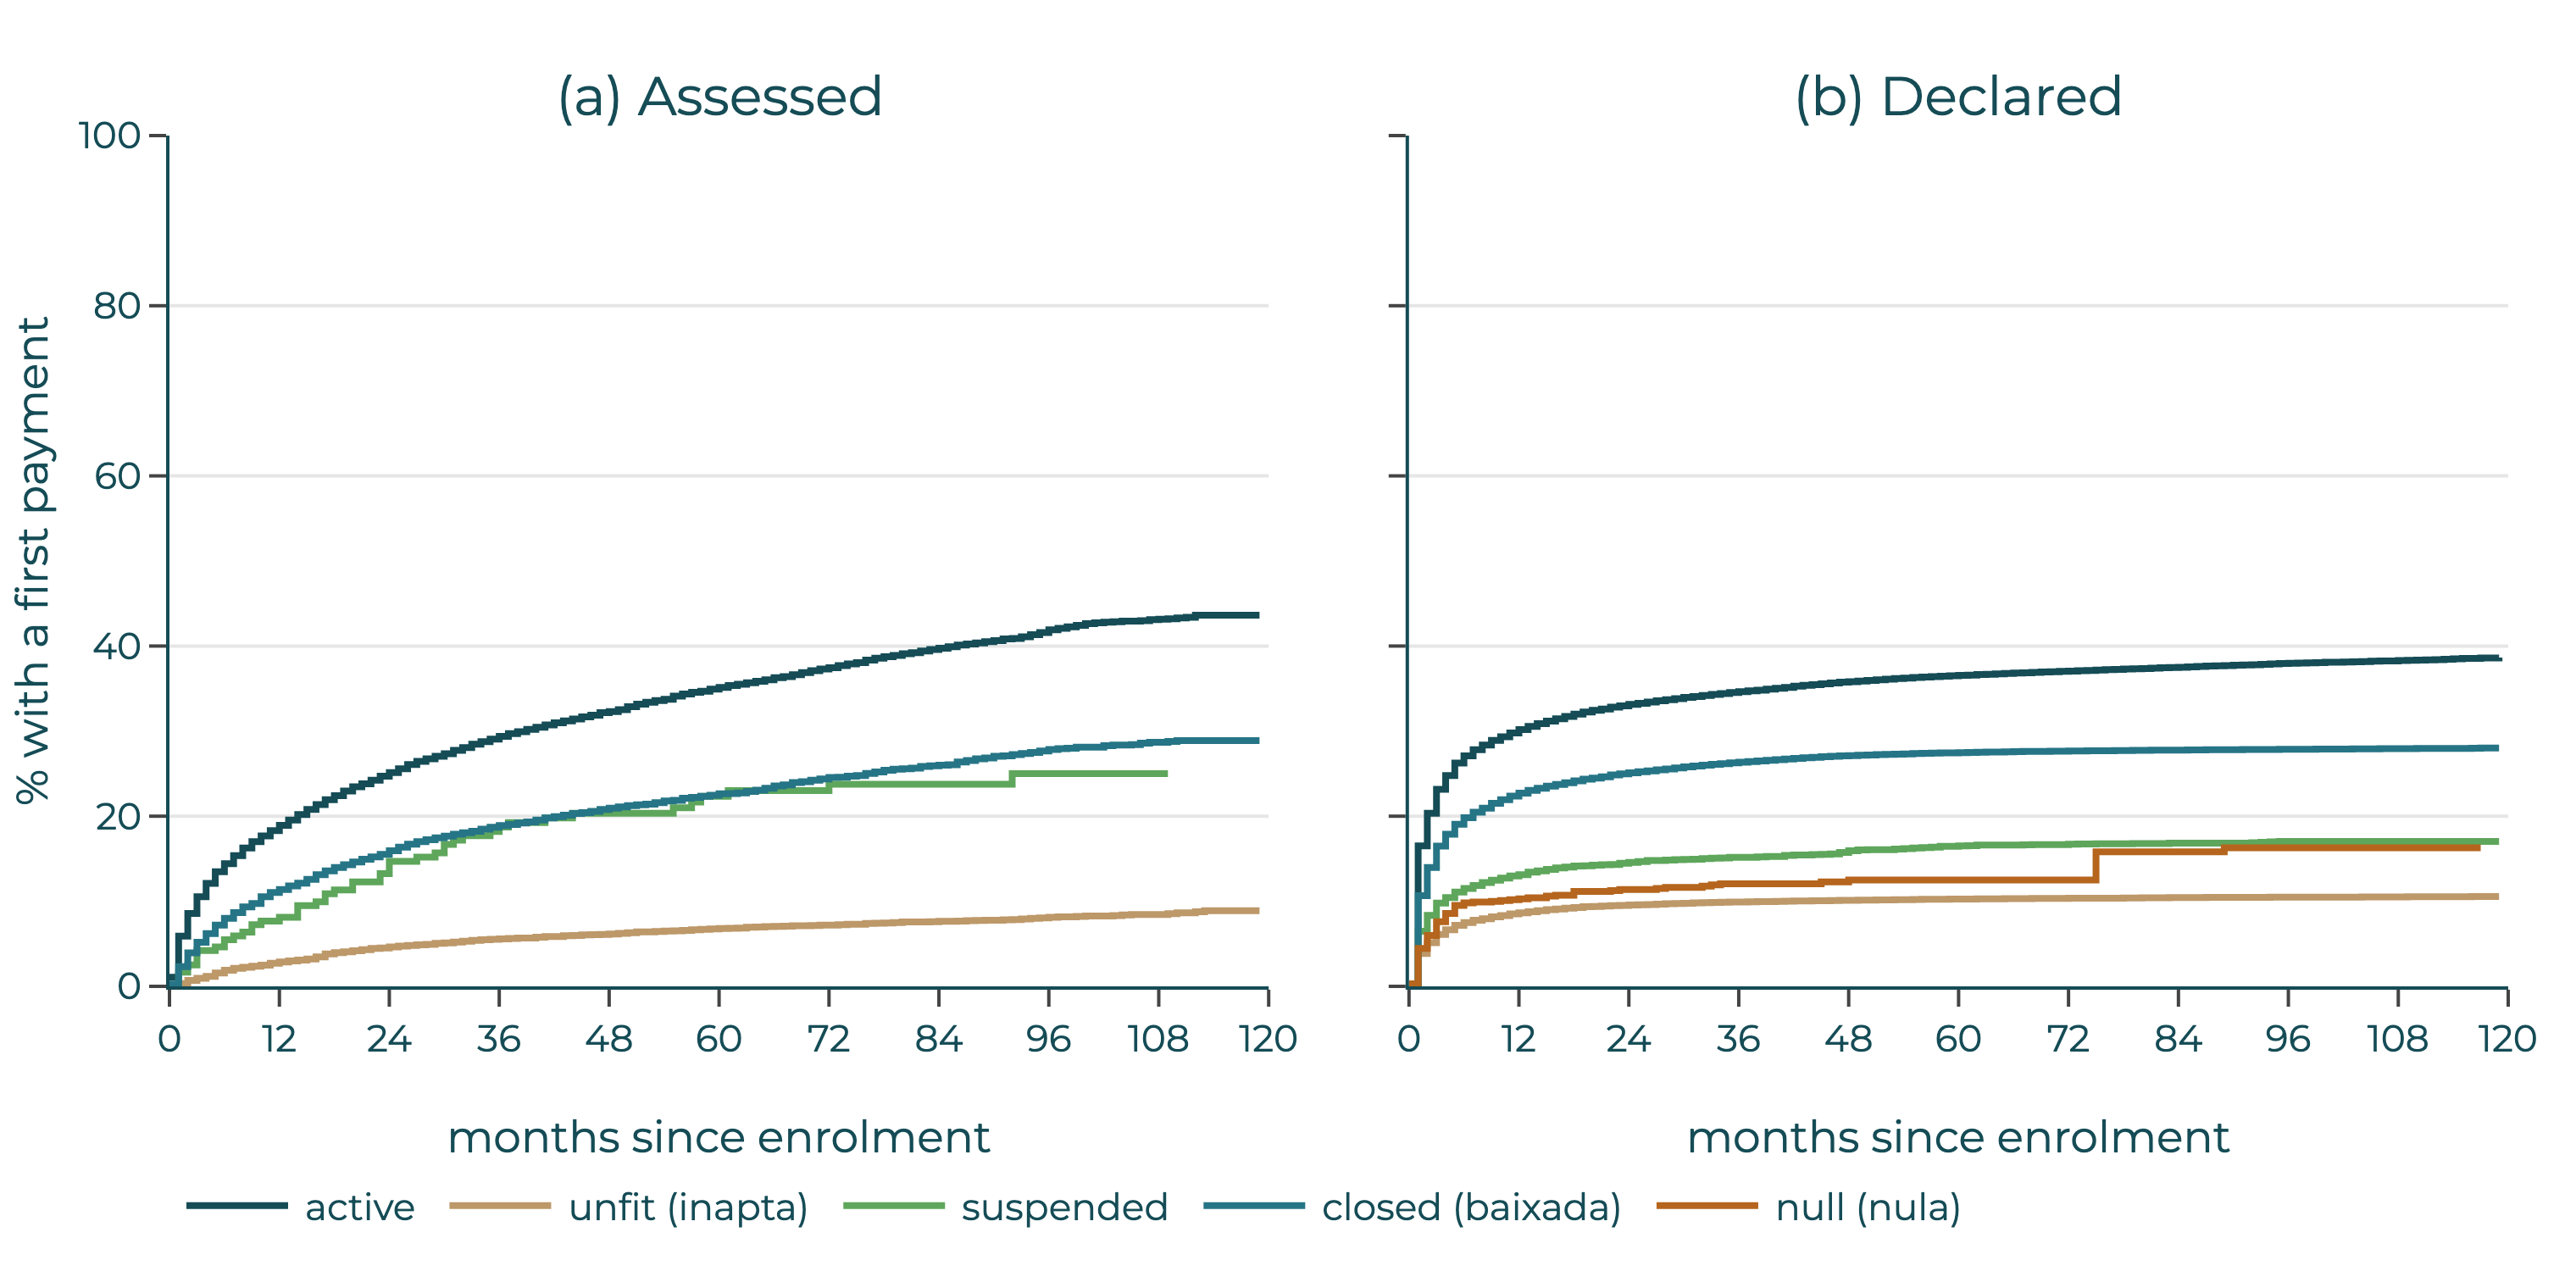
\includegraphics[width=\linewidth]{figures/fig_km_status_origin.png}
\caption{Kaplan--Meier share of CDAs with a first payment by months since enrolment, by registration status: assessed (a) and declared (b). Enrolment cohort 2016--2025.}\label{fig:km}
\end{figure}

\paragraph{Economic activity.}
The ten largest CNAE divisions hold \cnaeTenPctStock\% of the December 2025 \vat{} stock (Table~\ref{tab:cnae}).
The largest is division \cnaeTopDivision{} (\cnaeTopDivisionName), with \cnaeTopDivisionPctStock\% of the stock, \cnaeTopDivisionAssessedWeight\% of it assessed; the second is division \cnaeSecondDivision{} (\cnaeSecondDivisionName), with \cnaeSecondDivisionPctStock\%, \cnaeSecondDivisionAssessedWeight\% assessed.
Across the \cnaeNDivShown{} divisions shown, the assessed share of the stock ranges from \cnaeAssessedWeightMin\% to \cnaeAssessedWeightMax\%, and its Spearman correlation with the division's pooled recovery rate is \cnaeSpearman{} (Figure~\ref{fig:cnae}); this is an ecological description, not a within-division comparison.
\cnaeNDivSuppressed{} divisions are pooled for disclosure control.
\discutir{which divisions, if any, the text names and comments on}

\begin{table}[H]\centering\small
\caption{Ten largest CNAE 2.0 divisions by December 2025 \vat{} stock. Assessed weight: assessed share of the division's stock. Recovery: pooled 2016--2025 rate by origin. English names translated from the official Portuguese names. Descriptors only.}\label{tab:cnae}
\resizebox{\linewidth}{!}{% generated by projects/macro/notebooks/articles/icms_declarado_autuado.ipynb; do not edit by hand
% Ten largest CNAE divisions by December 2025 VAT (ICMS) stock: assessed weight and pooled 2016-2025 recovery by origin; descriptors only
\begin{tabular}{lrrrrr}
\toprule
division & activity (CNAE 2.0, English) & share of VAT stock (\%) & assessed weight (\%) & recovery, assessed (\%) & recovery, declared (\%) \\
\midrule
46 & Wholesale trade, except motor vehicles and motorcycles & 27.3 & 85.6 & 0.09 & 0.95 \\
47 & Retail trade & 11.8 & 72.5 & 0.13 & 1.44 \\
10 & Manufacture of food products & 6.6 & 82.4 & 0.12 & 1.56 \\
49 & Land transport & 5.6 & 43.1 & 0.28 & 1.19 \\
61 & Telecommunications & 4.2 & 96.5 & 0.33 & 1.85 \\
24 & Metallurgy & 4.0 & 86.5 & 0.06 & 0.86 \\
19 & Manufacture of coke, petroleum products and biofuels & 3.7 & 28.3 & 0.11 & 0.30 \\
82 & Office and administrative support services and other services mainly to businesses & 3.7 & 77.8 & 0.10 & 1.16 \\
22 & Manufacture of rubber and plastic products & 3.4 & 59.9 & 0.16 & 0.98 \\
25 & Manufacture of metal products, except machinery and equipment & 3.1 & 53.3 & 0.11 & 0.93 \\
\bottomrule
\end{tabular}
}
\end{table}

\begin{figure}[H]\centering
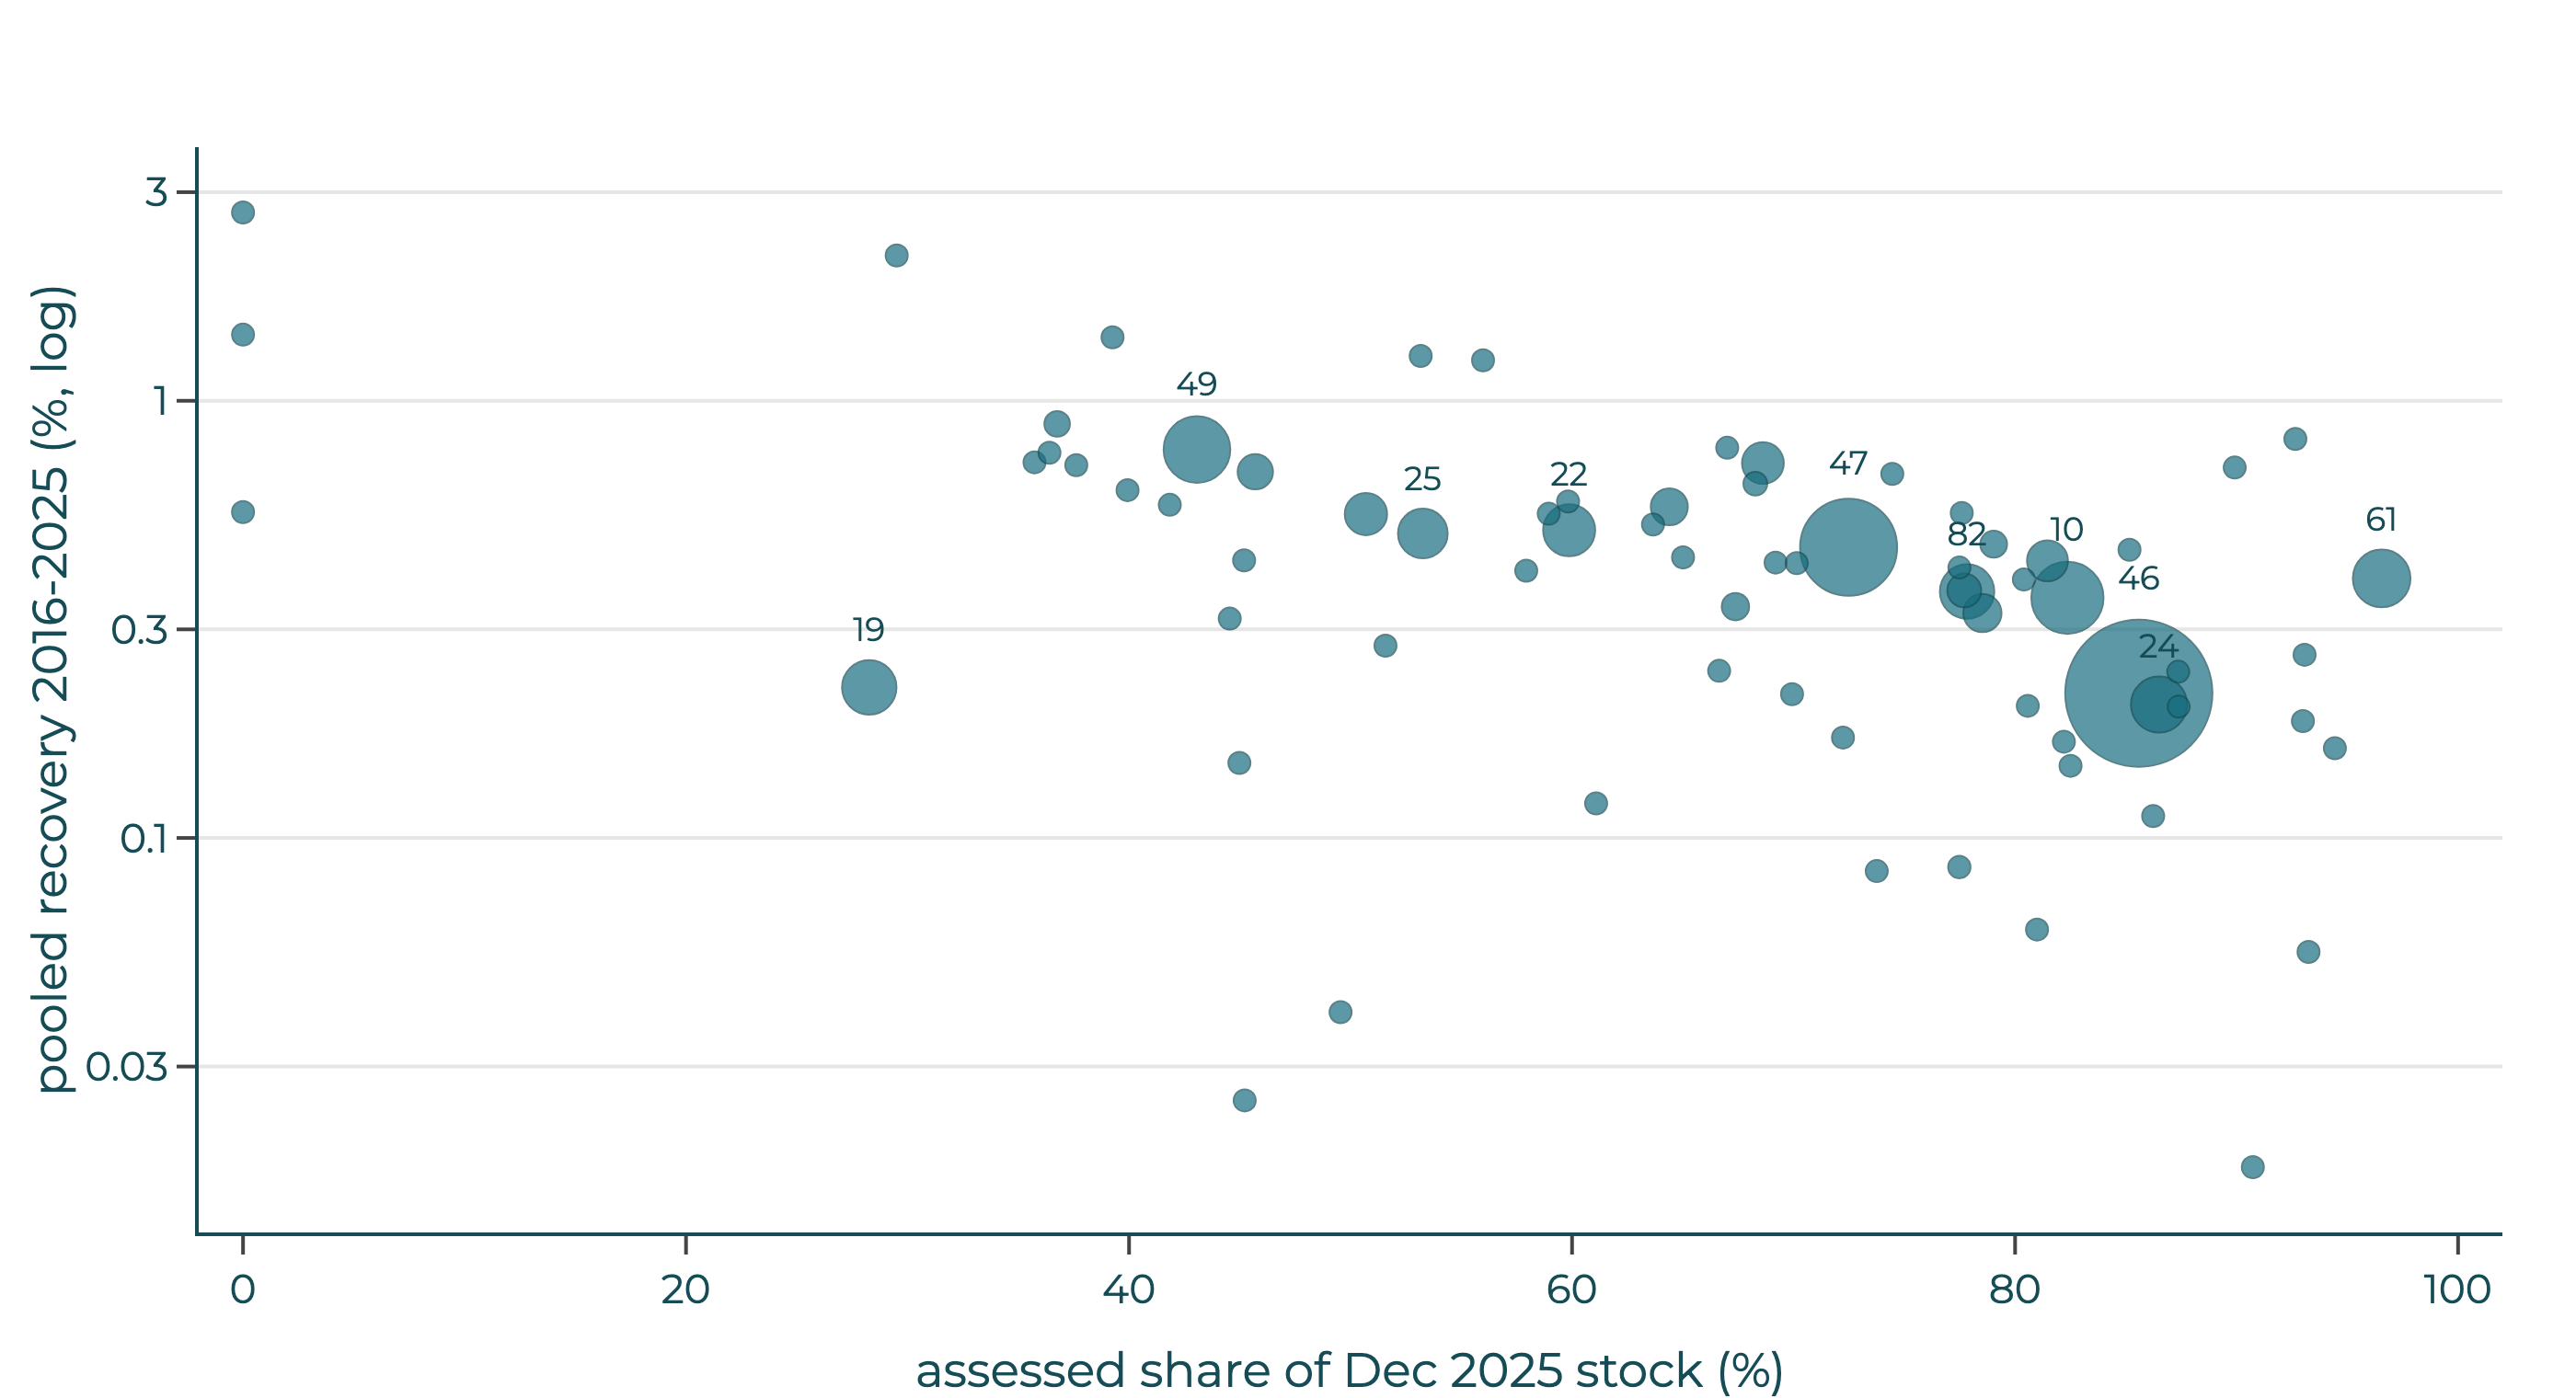
\includegraphics[width=0.85\linewidth]{figures/fig_cnae_division_origin.png}
\caption{CNAE divisions: assessed share of the December 2025 stock (horizontal) and pooled 2016--2025 recovery rate, log scale (vertical). Bubble area is proportional to the division's stock; the ten largest are labelled with their code.}\label{fig:cnae}
\end{figure}
